\documentclass[10pt]{article}
\usepackage{tmlr}
% camera-ready: \usepackage[accepted]{tmlr}   preprint: \usepackage[preprint]{tmlr}
%%%%% NEW MATH DEFINITIONS %%%%%

\usepackage{amsmath,amsfonts,bm}

% Mark sections of captions for referring to divisions of figures
\newcommand{\figleft}{{\em (Left)}}
\newcommand{\figcenter}{{\em (Center)}}
\newcommand{\figright}{{\em (Right)}}
\newcommand{\figtop}{{\em (Top)}}
\newcommand{\figbottom}{{\em (Bottom)}}
\newcommand{\captiona}{{\em (a)}}
\newcommand{\captionb}{{\em (b)}}
\newcommand{\captionc}{{\em (c)}}
\newcommand{\captiond}{{\em (d)}}

% Highlight a newly defined term
\newcommand{\newterm}[1]{{\bf #1}}


% Figure reference, lower-case.
\def\figref#1{figure~\ref{#1}}
% Figure reference, capital. For start of sentence
\def\Figref#1{Figure~\ref{#1}}
\def\twofigref#1#2{figures \ref{#1} and \ref{#2}}
\def\quadfigref#1#2#3#4{figures \ref{#1}, \ref{#2}, \ref{#3} and \ref{#4}}
% Section reference, lower-case.
\def\secref#1{section~\ref{#1}}
% Section reference, capital.
\def\Secref#1{Section~\ref{#1}}
% Reference to two sections.
\def\twosecrefs#1#2{sections \ref{#1} and \ref{#2}}
% Reference to three sections.
\def\secrefs#1#2#3{sections \ref{#1}, \ref{#2} and \ref{#3}}
% Reference to an equation, lower-case.
\def\eqref#1{equation~\ref{#1}}
% Reference to an equation, upper case
\def\Eqref#1{Equation~\ref{#1}}
% A raw reference to an equation---avoid using if possible
\def\plaineqref#1{\ref{#1}}
% Reference to a chapter, lower-case.
\def\chapref#1{chapter~\ref{#1}}
% Reference to an equation, upper case.
\def\Chapref#1{Chapter~\ref{#1}}
% Reference to a range of chapters
\def\rangechapref#1#2{chapters\ref{#1}--\ref{#2}}
% Reference to an algorithm, lower-case.
\def\algref#1{algorithm~\ref{#1}}
% Reference to an algorithm, upper case.
\def\Algref#1{Algorithm~\ref{#1}}
\def\twoalgref#1#2{algorithms \ref{#1} and \ref{#2}}
\def\Twoalgref#1#2{Algorithms \ref{#1} and \ref{#2}}
% Reference to a part, lower case
\def\partref#1{part~\ref{#1}}
% Reference to a part, upper case
\def\Partref#1{Part~\ref{#1}}
\def\twopartref#1#2{parts \ref{#1} and \ref{#2}}

\def\ceil#1{\lceil #1 \rceil}
\def\floor#1{\lfloor #1 \rfloor}
\def\1{\bm{1}}
\newcommand{\train}{\mathcal{D}}
\newcommand{\valid}{\mathcal{D_{\mathrm{valid}}}}
\newcommand{\test}{\mathcal{D_{\mathrm{test}}}}

\def\eps{{\epsilon}}


% Random variables
\def\reta{{\textnormal{$\eta$}}}
\def\ra{{\textnormal{a}}}
\def\rb{{\textnormal{b}}}
\def\rc{{\textnormal{c}}}
\def\rd{{\textnormal{d}}}
\def\re{{\textnormal{e}}}
\def\rf{{\textnormal{f}}}
\def\rg{{\textnormal{g}}}
\def\rh{{\textnormal{h}}}
\def\ri{{\textnormal{i}}}
\def\rj{{\textnormal{j}}}
\def\rk{{\textnormal{k}}}
\def\rl{{\textnormal{l}}}
% rm is already a command, just don't name any random variables m
\def\rn{{\textnormal{n}}}
\def\ro{{\textnormal{o}}}
\def\rp{{\textnormal{p}}}
\def\rq{{\textnormal{q}}}
\def\rr{{\textnormal{r}}}
\def\rs{{\textnormal{s}}}
\def\rt{{\textnormal{t}}}
\def\ru{{\textnormal{u}}}
\def\rv{{\textnormal{v}}}
\def\rw{{\textnormal{w}}}
\def\rx{{\textnormal{x}}}
\def\ry{{\textnormal{y}}}
\def\rz{{\textnormal{z}}}

% Random vectors
\def\rvepsilon{{\mathbf{\epsilon}}}
\def\rvtheta{{\mathbf{\theta}}}
\def\rva{{\mathbf{a}}}
\def\rvb{{\mathbf{b}}}
\def\rvc{{\mathbf{c}}}
\def\rvd{{\mathbf{d}}}
\def\rve{{\mathbf{e}}}
\def\rvf{{\mathbf{f}}}
\def\rvg{{\mathbf{g}}}
\def\rvh{{\mathbf{h}}}
\def\rvu{{\mathbf{i}}}
\def\rvj{{\mathbf{j}}}
\def\rvk{{\mathbf{k}}}
\def\rvl{{\mathbf{l}}}
\def\rvm{{\mathbf{m}}}
\def\rvn{{\mathbf{n}}}
\def\rvo{{\mathbf{o}}}
\def\rvp{{\mathbf{p}}}
\def\rvq{{\mathbf{q}}}
\def\rvr{{\mathbf{r}}}
\def\rvs{{\mathbf{s}}}
\def\rvt{{\mathbf{t}}}
\def\rvu{{\mathbf{u}}}
\def\rvv{{\mathbf{v}}}
\def\rvw{{\mathbf{w}}}
\def\rvx{{\mathbf{x}}}
\def\rvy{{\mathbf{y}}}
\def\rvz{{\mathbf{z}}}

% Elements of random vectors
\def\erva{{\textnormal{a}}}
\def\ervb{{\textnormal{b}}}
\def\ervc{{\textnormal{c}}}
\def\ervd{{\textnormal{d}}}
\def\erve{{\textnormal{e}}}
\def\ervf{{\textnormal{f}}}
\def\ervg{{\textnormal{g}}}
\def\ervh{{\textnormal{h}}}
\def\ervi{{\textnormal{i}}}
\def\ervj{{\textnormal{j}}}
\def\ervk{{\textnormal{k}}}
\def\ervl{{\textnormal{l}}}
\def\ervm{{\textnormal{m}}}
\def\ervn{{\textnormal{n}}}
\def\ervo{{\textnormal{o}}}
\def\ervp{{\textnormal{p}}}
\def\ervq{{\textnormal{q}}}
\def\ervr{{\textnormal{r}}}
\def\ervs{{\textnormal{s}}}
\def\ervt{{\textnormal{t}}}
\def\ervu{{\textnormal{u}}}
\def\ervv{{\textnormal{v}}}
\def\ervw{{\textnormal{w}}}
\def\ervx{{\textnormal{x}}}
\def\ervy{{\textnormal{y}}}
\def\ervz{{\textnormal{z}}}

% Random matrices
\def\rmA{{\mathbf{A}}}
\def\rmB{{\mathbf{B}}}
\def\rmC{{\mathbf{C}}}
\def\rmD{{\mathbf{D}}}
\def\rmE{{\mathbf{E}}}
\def\rmF{{\mathbf{F}}}
\def\rmG{{\mathbf{G}}}
\def\rmH{{\mathbf{H}}}
\def\rmI{{\mathbf{I}}}
\def\rmJ{{\mathbf{J}}}
\def\rmK{{\mathbf{K}}}
\def\rmL{{\mathbf{L}}}
\def\rmM{{\mathbf{M}}}
\def\rmN{{\mathbf{N}}}
\def\rmO{{\mathbf{O}}}
\def\rmP{{\mathbf{P}}}
\def\rmQ{{\mathbf{Q}}}
\def\rmR{{\mathbf{R}}}
\def\rmS{{\mathbf{S}}}
\def\rmT{{\mathbf{T}}}
\def\rmU{{\mathbf{U}}}
\def\rmV{{\mathbf{V}}}
\def\rmW{{\mathbf{W}}}
\def\rmX{{\mathbf{X}}}
\def\rmY{{\mathbf{Y}}}
\def\rmZ{{\mathbf{Z}}}

% Elements of random matrices
\def\ermA{{\textnormal{A}}}
\def\ermB{{\textnormal{B}}}
\def\ermC{{\textnormal{C}}}
\def\ermD{{\textnormal{D}}}
\def\ermE{{\textnormal{E}}}
\def\ermF{{\textnormal{F}}}
\def\ermG{{\textnormal{G}}}
\def\ermH{{\textnormal{H}}}
\def\ermI{{\textnormal{I}}}
\def\ermJ{{\textnormal{J}}}
\def\ermK{{\textnormal{K}}}
\def\ermL{{\textnormal{L}}}
\def\ermM{{\textnormal{M}}}
\def\ermN{{\textnormal{N}}}
\def\ermO{{\textnormal{O}}}
\def\ermP{{\textnormal{P}}}
\def\ermQ{{\textnormal{Q}}}
\def\ermR{{\textnormal{R}}}
\def\ermS{{\textnormal{S}}}
\def\ermT{{\textnormal{T}}}
\def\ermU{{\textnormal{U}}}
\def\ermV{{\textnormal{V}}}
\def\ermW{{\textnormal{W}}}
\def\ermX{{\textnormal{X}}}
\def\ermY{{\textnormal{Y}}}
\def\ermZ{{\textnormal{Z}}}

% Vectors
\def\vzero{{\bm{0}}}
\def\vone{{\bm{1}}}
\def\vmu{{\bm{\mu}}}
\def\vtheta{{\bm{\theta}}}
\def\va{{\bm{a}}}
\def\vb{{\bm{b}}}
\def\vc{{\bm{c}}}
\def\vd{{\bm{d}}}
\def\ve{{\bm{e}}}
\def\vf{{\bm{f}}}
\def\vg{{\bm{g}}}
\def\vh{{\bm{h}}}
\def\vi{{\bm{i}}}
\def\vj{{\bm{j}}}
\def\vk{{\bm{k}}}
\def\vl{{\bm{l}}}
\def\vm{{\bm{m}}}
\def\vn{{\bm{n}}}
\def\vo{{\bm{o}}}
\def\vp{{\bm{p}}}
\def\vq{{\bm{q}}}
\def\vr{{\bm{r}}}
\def\vs{{\bm{s}}}
\def\vt{{\bm{t}}}
\def\vu{{\bm{u}}}
\def\vv{{\bm{v}}}
\def\vw{{\bm{w}}}
\def\vx{{\bm{x}}}
\def\vy{{\bm{y}}}
\def\vz{{\bm{z}}}

% Elements of vectors
\def\evalpha{{\alpha}}
\def\evbeta{{\beta}}
\def\evepsilon{{\epsilon}}
\def\evlambda{{\lambda}}
\def\evomega{{\omega}}
\def\evmu{{\mu}}
\def\evpsi{{\psi}}
\def\evsigma{{\sigma}}
\def\evtheta{{\theta}}
\def\eva{{a}}
\def\evb{{b}}
\def\evc{{c}}
\def\evd{{d}}
\def\eve{{e}}
\def\evf{{f}}
\def\evg{{g}}
\def\evh{{h}}
\def\evi{{i}}
\def\evj{{j}}
\def\evk{{k}}
\def\evl{{l}}
\def\evm{{m}}
\def\evn{{n}}
\def\evo{{o}}
\def\evp{{p}}
\def\evq{{q}}
\def\evr{{r}}
\def\evs{{s}}
\def\evt{{t}}
\def\evu{{u}}
\def\evv{{v}}
\def\evw{{w}}
\def\evx{{x}}
\def\evy{{y}}
\def\evz{{z}}

% Matrix
\def\mA{{\bm{A}}}
\def\mB{{\bm{B}}}
\def\mC{{\bm{C}}}
\def\mD{{\bm{D}}}
\def\mE{{\bm{E}}}
\def\mF{{\bm{F}}}
\def\mG{{\bm{G}}}
\def\mH{{\bm{H}}}
\def\mI{{\bm{I}}}
\def\mJ{{\bm{J}}}
\def\mK{{\bm{K}}}
\def\mL{{\bm{L}}}
\def\mM{{\bm{M}}}
\def\mN{{\bm{N}}}
\def\mO{{\bm{O}}}
\def\mP{{\bm{P}}}
\def\mQ{{\bm{Q}}}
\def\mR{{\bm{R}}}
\def\mS{{\bm{S}}}
\def\mT{{\bm{T}}}
\def\mU{{\bm{U}}}
\def\mV{{\bm{V}}}
\def\mW{{\bm{W}}}
\def\mX{{\bm{X}}}
\def\mY{{\bm{Y}}}
\def\mZ{{\bm{Z}}}
\def\mBeta{{\bm{\beta}}}
\def\mPhi{{\bm{\Phi}}}
\def\mLambda{{\bm{\Lambda}}}
\def\mSigma{{\bm{\Sigma}}}

% Tensor
\DeclareMathAlphabet{\mathsfit}{\encodingdefault}{\sfdefault}{m}{sl}
\SetMathAlphabet{\mathsfit}{bold}{\encodingdefault}{\sfdefault}{bx}{n}
\newcommand{\tens}[1]{\bm{\mathsfit{#1}}}
\def\tA{{\tens{A}}}
\def\tB{{\tens{B}}}
\def\tC{{\tens{C}}}
\def\tD{{\tens{D}}}
\def\tE{{\tens{E}}}
\def\tF{{\tens{F}}}
\def\tG{{\tens{G}}}
\def\tH{{\tens{H}}}
\def\tI{{\tens{I}}}
\def\tJ{{\tens{J}}}
\def\tK{{\tens{K}}}
\def\tL{{\tens{L}}}
\def\tM{{\tens{M}}}
\def\tN{{\tens{N}}}
\def\tO{{\tens{O}}}
\def\tP{{\tens{P}}}
\def\tQ{{\tens{Q}}}
\def\tR{{\tens{R}}}
\def\tS{{\tens{S}}}
\def\tT{{\tens{T}}}
\def\tU{{\tens{U}}}
\def\tV{{\tens{V}}}
\def\tW{{\tens{W}}}
\def\tX{{\tens{X}}}
\def\tY{{\tens{Y}}}
\def\tZ{{\tens{Z}}}


% Graph
\def\gA{{\mathcal{A}}}
\def\gB{{\mathcal{B}}}
\def\gC{{\mathcal{C}}}
\def\gD{{\mathcal{D}}}
\def\gE{{\mathcal{E}}}
\def\gF{{\mathcal{F}}}
\def\gG{{\mathcal{G}}}
\def\gH{{\mathcal{H}}}
\def\gI{{\mathcal{I}}}
\def\gJ{{\mathcal{J}}}
\def\gK{{\mathcal{K}}}
\def\gL{{\mathcal{L}}}
\def\gM{{\mathcal{M}}}
\def\gN{{\mathcal{N}}}
\def\gO{{\mathcal{O}}}
\def\gP{{\mathcal{P}}}
\def\gQ{{\mathcal{Q}}}
\def\gR{{\mathcal{R}}}
\def\gS{{\mathcal{S}}}
\def\gT{{\mathcal{T}}}
\def\gU{{\mathcal{U}}}
\def\gV{{\mathcal{V}}}
\def\gW{{\mathcal{W}}}
\def\gX{{\mathcal{X}}}
\def\gY{{\mathcal{Y}}}
\def\gZ{{\mathcal{Z}}}

% Sets
\def\sA{{\mathbb{A}}}
\def\sB{{\mathbb{B}}}
\def\sC{{\mathbb{C}}}
\def\sD{{\mathbb{D}}}
% Don't use a set called E, because this would be the same as our symbol
% for expectation.
\def\sF{{\mathbb{F}}}
\def\sG{{\mathbb{G}}}
\def\sH{{\mathbb{H}}}
\def\sI{{\mathbb{I}}}
\def\sJ{{\mathbb{J}}}
\def\sK{{\mathbb{K}}}
\def\sL{{\mathbb{L}}}
\def\sM{{\mathbb{M}}}
\def\sN{{\mathbb{N}}}
\def\sO{{\mathbb{O}}}
\def\sP{{\mathbb{P}}}
\def\sQ{{\mathbb{Q}}}
\def\sR{{\mathbb{R}}}
\def\sS{{\mathbb{S}}}
\def\sT{{\mathbb{T}}}
\def\sU{{\mathbb{U}}}
\def\sV{{\mathbb{V}}}
\def\sW{{\mathbb{W}}}
\def\sX{{\mathbb{X}}}
\def\sY{{\mathbb{Y}}}
\def\sZ{{\mathbb{Z}}}

% Entries of a matrix
\def\emLambda{{\Lambda}}
\def\emA{{A}}
\def\emB{{B}}
\def\emC{{C}}
\def\emD{{D}}
\def\emE{{E}}
\def\emF{{F}}
\def\emG{{G}}
\def\emH{{H}}
\def\emI{{I}}
\def\emJ{{J}}
\def\emK{{K}}
\def\emL{{L}}
\def\emM{{M}}
\def\emN{{N}}
\def\emO{{O}}
\def\emP{{P}}
\def\emQ{{Q}}
\def\emR{{R}}
\def\emS{{S}}
\def\emT{{T}}
\def\emU{{U}}
\def\emV{{V}}
\def\emW{{W}}
\def\emX{{X}}
\def\emY{{Y}}
\def\emZ{{Z}}
\def\emSigma{{\Sigma}}

% entries of a tensor
% Same font as tensor, without \bm wrapper
\newcommand{\etens}[1]{\mathsfit{#1}}
\def\etLambda{{\etens{\Lambda}}}
\def\etA{{\etens{A}}}
\def\etB{{\etens{B}}}
\def\etC{{\etens{C}}}
\def\etD{{\etens{D}}}
\def\etE{{\etens{E}}}
\def\etF{{\etens{F}}}
\def\etG{{\etens{G}}}
\def\etH{{\etens{H}}}
\def\etI{{\etens{I}}}
\def\etJ{{\etens{J}}}
\def\etK{{\etens{K}}}
\def\etL{{\etens{L}}}
\def\etM{{\etens{M}}}
\def\etN{{\etens{N}}}
\def\etO{{\etens{O}}}
\def\etP{{\etens{P}}}
\def\etQ{{\etens{Q}}}
\def\etR{{\etens{R}}}
\def\etS{{\etens{S}}}
\def\etT{{\etens{T}}}
\def\etU{{\etens{U}}}
\def\etV{{\etens{V}}}
\def\etW{{\etens{W}}}
\def\etX{{\etens{X}}}
\def\etY{{\etens{Y}}}
\def\etZ{{\etens{Z}}}

% The true underlying data generating distribution
\newcommand{\pdata}{p_{\rm{data}}}
% The empirical distribution defined by the training set
\newcommand{\ptrain}{\hat{p}_{\rm{data}}}
\newcommand{\Ptrain}{\hat{P}_{\rm{data}}}
% The model distribution
\newcommand{\pmodel}{p_{\rm{model}}}
\newcommand{\Pmodel}{P_{\rm{model}}}
\newcommand{\ptildemodel}{\tilde{p}_{\rm{model}}}
% Stochastic autoencoder distributions
\newcommand{\pencode}{p_{\rm{encoder}}}
\newcommand{\pdecode}{p_{\rm{decoder}}}
\newcommand{\precons}{p_{\rm{reconstruct}}}

\newcommand{\laplace}{\mathrm{Laplace}} % Laplace distribution

\newcommand{\E}{\mathbb{E}}
\newcommand{\Ls}{\mathcal{L}}
\newcommand{\R}{\mathbb{R}}
\newcommand{\emp}{\tilde{p}}
\newcommand{\lr}{\alpha}
\newcommand{\reg}{\lambda}
\newcommand{\rect}{\mathrm{rectifier}}
\newcommand{\softmax}{\mathrm{softmax}}
\newcommand{\sigmoid}{\sigma}
\newcommand{\softplus}{\zeta}
\newcommand{\KL}{D_{\mathrm{KL}}}
\newcommand{\Var}{\mathrm{Var}}
\newcommand{\standarderror}{\mathrm{SE}}
\newcommand{\Cov}{\mathrm{Cov}}
% Wolfram Mathworld says $L^2$ is for function spaces and $\ell^2$ is for vectors
% But then they seem to use $L^2$ for vectors throughout the site, and so does
% wikipedia.
\newcommand{\normlzero}{L^0}
\newcommand{\normlone}{L^1}
\newcommand{\normltwo}{L^2}
\newcommand{\normlp}{L^p}
\newcommand{\normmax}{L^\infty}

\newcommand{\parents}{Pa} % See usage in notation.tex. Chosen to match Daphne's book.

\DeclareMathOperator*{\argmax}{arg\,max}
\DeclareMathOperator*{\argmin}{arg\,min}

\DeclareMathOperator{\sign}{sign}
\DeclareMathOperator{\Tr}{Tr}
\let\ab\allowbreak

\usepackage{hyperref}
\usepackage{url}
\usepackage{booktabs,longtable,graphicx,amsmath,amssymb,enumitem}

\title{Compressed embeddings fail unevenly across languages:\\the score margin, not the calibration language, decides}

\author{\name Anonymous \email anonymous@example.com \\
      \addr Independent researcher}

\def\month{MM}
\def\year{YYYY}
\def\openreview{\url{https://openreview.net/forum?id=XXXX}}

\begin{document}
\maketitle

\begin{abstract}
Search on phones and laptops stores each document as an embedding vector, and to save memory the vectors are stored at 8, 4, 2 or 1 bit per dimension instead of 32. The evidence that this costs little comes from English. We measure the retrieval loss of float16, float8, int8, int4, int2 and binary storage in 122 languages with identical content (Belebele) for five multilingual embedding models under 600M parameters, and repeat the protocol on a second task with 28 times larger corpora. At 8 and 4 bits nothing is lost in any language. Below that, the loss is uneven in every model: English loses least and low-resource languages most. How much is lost, however, is decided by the model rather than by the bit width: the three multilingual-E5 models lose 7--71\% of nDCG@10 under 1-bit storage, while BGE-M3 and Qwen3-Embedding lose under 5\% in any language at the same 1024 dimensions. One quantity, computable at float32 before deployment, explains this: the score margin between the relevant document and the best wrong one. It orders the languages within every model (Spearman $\rho$ from $-0.81$ to $-0.98$), explains three quarters of the variance across models and languages, and makes tokenizer fertility, script and resource class redundant. The presumed cause, calibrating the number ranges on English text, is not the cause: calibrating on other languages changes the loss by at most 3.2 points. What works is changing the estimator, not its language: percentile clipping halves the 2-bit loss, and subtracting the calibration mean before compression, one vector fitted on English, raises the margins of the E5 models fourfold and cuts their 1-bit loss from 27--71\% to under 4\% in every language group. Rescoring 100 candidates with an int8 copy of the corpus achieves less at nine times the storage. Code and per-language results are released.
\end{abstract}

\section{Introduction}
Dense retrieval represents every document as a vector, the embedding, and answers a query by finding the documents whose vectors score highest against the query's vector. On a phone or a laptop the vectors of the whole corpus sit in memory, so they are stored at reduced precision: float16 or int8 by default, and 4, 2 or 1 bit per dimension when memory is tight \citep{shakir2024quant,yamada2021bpr}. A 1-bit vector takes a thirty-second of the space of a float32 one. Recent measurements on the MTEB benchmark \citep{muennighoff2023mteb} say this is nearly free: float8 loses under 0.3\% of retrieval quality \citep{sanchez2025storage}, and combined with dimensionality reduction embeddings compress to a fraction of a percent of their size with little loss \citep{dimquant2026}. Both measurements use English models on English data.

Multilingual embedding models serve users whose languages the models handle less well than English. That raises three questions which this paper answers.
\begin{enumerate}[nosep]
\item Does compression cost some languages more than others?
\item If so, is the cause the \emph{calibration data}? Integer formats need a number range per dimension, and practitioners estimate it on English text.
\item If the calibration language is not the cause, what is, and what can be done about it?
\end{enumerate}
We answer them on a benchmark whose content is the same in all 122 languages, so that a difference between two languages is a difference in how the model embeds them, not a difference in the task. We then check the answers on a second task with much larger corpora, and we test the two fixes that the answers suggest.

\paragraph{Findings.} Each is supported by a table or figure in the section cited.
\begin{enumerate}[nosep]
\item \textbf{The loss is uneven, in every model.} At 8 and 4 bits no language loses more than about 3\%. Below that, English loses least, the average language more, and low-resource languages most, in all five models and all formats. For the E5 models 98--99\% of languages lose more than English (Section~\ref{sec:uneven}).
\item \textbf{How much is lost is a property of the model, not of the bit width or the dimensionality.} Under 1-bit storage, the E5 family loses 27--71\% (small), 8--40\% (base) and 7--38\% (large), the two numbers being English and low-resource languages; BGE-M3 and Qwen3-Embedding lose 1--4\%. E5-large has the same 1024 dimensions as the two robust models (Section~\ref{sec:model}).
\item \textbf{The float32 score margin explains the loss.} The margin between the relevant document and the best distractor orders the languages within every model ($\rho$ from $-0.81$ to $-0.98$) and explains three quarters of the variance across models and languages. Which languages have thin margins is the same in every model ($\rho\ge0.90$ between models); how thin they are depends on how spread out the model's embedding space is. Tokenizer fertility, script and resource class are each predictive on their own but add almost nothing once the margin is known. Six languages available both in their native script and romanised show the effect without any change of content (Section~\ref{sec:margin}).
\item \textbf{The calibration language is not the cause.} Replacing English calibration by a sample from all other languages, excluding the target, changes the loss by at most 3.2 points. Replacing the range estimator matters far more: clipping the range to percentiles halves the 2-bit loss (Section~\ref{sec:calib}).
\item \textbf{Subtracting the mean removes most of the loss.} Centring the vectors on the calibration mean, one vector fitted on English and applied unchanged to all 122 languages, raises the E5 margins fourfold, improves their float32 quality, and cuts their 1-bit loss relative to the original float32 quality from 59\% to 4\% on average and from 71\% to 2\% on low-resource languages. Full whitening on 1388 vectors overfits (Section~\ref{sec:whiten}).
\item \textbf{Rescoring helps less per byte.} Rescoring the top 100 binary candidates with an int8 corpus still leaves 9--13\% for E5-small, while 20 candidates suffice for the robust models (Section~\ref{sec:rescore}).
\item \textbf{The ordering holds on larger corpora.} On a Wikipedia retrieval task with 13{,}500 documents per language the ordering of models is unchanged and the losses are equal or smaller (Section~\ref{sec:wiki}).
\end{enumerate}

\section{Background and terms}\label{sec:terms}
This section fixes the vocabulary used in the rest of the paper.

\textbf{Retrieval and nDCG@10.} A corpus holds $n$ documents with unit-norm embeddings $\vd_1,\dots,\vd_n\in\R^d$. A query with embedding $\vq$ scores every document by the dot product $s(\vq,\vd_i)=\vq^\top\vd_i$ and returns the ten highest. nDCG@10 is 1 if the relevant document is ranked first, $1/\log_2(r+1)$ if it is ranked $r\le10$, and 0 otherwise, averaged over queries. All tasks here have exactly one relevant document per query.

\textbf{Compression formats.} A float32 vector uses 32 bits per dimension. \emph{float16} and \emph{float8} are shorter floating-point formats. \emph{int$b$} maps each dimension to one of $2^b$ evenly spaced levels between a lower and an upper bound $l_j,u_j$; the bounds are the \emph{range}. \emph{Binary} keeps one bit per dimension: the sign of the value, or the sign after subtracting a threshold. Every format is applied after the model has produced the float32 vector; the model itself is never changed.

\textbf{Calibration.} The ranges of int$b$ and the thresholds of binary storage are estimated from a sample of embeddings, the \emph{calibration set}. The range \emph{estimator} is the rule that turns the sample into bounds: the minimum and maximum of the sample, or a pair of percentiles.

\textbf{Relative loss.} For a language and a format, loss is $(\mathrm{nDCG}_{32}-\mathrm{nDCG}_{b})/\mathrm{nDCG}_{32}$ in percent, where $\mathrm{nDCG}_{32}$ is the float32 quality of the same model on the same language. A loss of 50\% means half of the retrieval quality is gone.

\textbf{Margin.} For one query, the margin is the float32 score of the relevant document minus the highest score among the other documents. It is positive exactly when the relevant document is ranked first, and its size is the amount of score noise the ranking can absorb before it flips. The margin of a language is the mean over its queries.

\textbf{Low-resource.} We use the 0--5 resource classes of \citet{joshi2020state}, which rank languages by the labelled and unlabelled data available for them. Classes 0--1 are called low-resource; 47 of the 122 languages fall there.

\section{Related work}
\paragraph{Embedding compression.} Product quantisation \citep{jegou2011pq} and its descendants in Faiss \citep{johnson2019faiss} compress vectors for approximate search with learned codebooks. The formats studied here are the simpler scalar ones that on-device libraries and vector databases expose directly: per-dimension integer quantisation and sign binarisation, popularised for sentence embeddings by \citet{shakir2024quant} together with a float rescoring step, and binary passage retrieval with hashing \citep{yamada2021bpr}. Matryoshka representation learning \citep{kusupati2022matryoshka} reduces the number of dimensions instead of their precision and is orthogonal to our setting. \citet{sanchez2025storage} and \citet{dimquant2026} measure scalar formats and dimensionality reduction on MTEB with English models. We extend the measurement to 122 languages and five multilingual models and ask what predicts the per-language loss.

\paragraph{Quantisation and languages.} \citet{marchisio2024quantization} show that quantising the \emph{weights} of multilingual large language models degrades non-Latin-script and low-resource languages more than English, and that automatic metrics understate the damage. We study a different object, the stored embedding rather than the model, and find the same direction of inequality with an explanation that can be measured directly: the geometry of the embedding space per language.

\paragraph{Anisotropy and whitening.} Contextual embeddings occupy a narrow cone of the space \citep{ethayarajh2019contextual,gao2019representation}, also in multilingual encoders \citep{rajaee2022isotropy}. Post-hoc corrections such as flow-based transforms \citep{li2020bertflow} and whitening \citep{su2021whitening} spread the space and improve semantic similarity. We connect anisotropy to compression: a narrow cone leaves small score margins, and quantisation noise flips rankings where margins are small. This makes centring and whitening natural candidates for reducing the loss, which we test.

\paragraph{Tokenizer fertility.} The number of subword tokens a tokenizer needs per word or per sentence differs by language and predicts downstream quality \citep{rust2021tokenizer}. We use fertility as one of three language covariates and find that it acts through the margin.

\section{Method}
\subsection{Storage formats}
Let $\vx\in\R^d$ be a unit-norm embedding and $\mathcal{C}\subset\R^d$ a calibration set. We evaluate, all post hoc:
\begin{itemize}[nosep]
\item \textbf{float16} and \textbf{float8} (E4M3): direct casts.
\item \textbf{int$b$}, $b\in\{8,4,2\}$: $q_j=\mathrm{round}\big((x_j-l_j)/s_j\big)$ with step $s_j=(u_j-l_j)/(2^b-1)$, where $[l_j,u_j]$ is either the minimum and maximum of dimension $j$ over $\mathcal{C}$, the recipe of \citet{shakir2024quant}, or its 5th and 95th percentiles, which we call \textbf{clip}. Values outside the range are clipped to it.
\item \textbf{binary}: $\mathrm{sign}(x_j-t_j)$ with $t_j=0$ (\textbf{sign}) or $t_j$ the mean of dimension $j$ over $\mathcal{C}$ (\textbf{centred}).
\end{itemize}
Scores are dot products between the dequantised corpus vector and the query. In the main results the query stays float32, the on-device situation where the corpus is stored compressed and the query is embedded at search time. The symmetric case, query compressed the same way, is in Appendix~\ref{app:sym}.

\subsection{Calibration sources}\label{sec:calsources}
Every calibrated format is run with five sources of $\mathcal{C}$, all of 1388 vectors unless stated: (a) \textbf{English}: English documents and queries; (b) \textbf{mixed}: a uniform sample over the 121 other languages, always excluding the language being evaluated; (c) \textbf{Latin-only}: the same, restricted to Latin-script languages other than the target; (d) \textbf{target, 64}: 64 target-language texts; (e) \textbf{target, all}: all 1388 target-language texts, an oracle that overlaps the evaluation set and serves as an upper bound.

\subsection{Margin and covariates}
The margin of query $q$ is $m(q)=s(\vq,\vd^+)-\max_{i\ne +}s(\vq,\vd_i)$ at float32; the margin of a language is its mean over queries. Language covariates are tokenizer \textbf{fertility} (tokens per document divided by the English count for the same documents, so a value of 2 means twice as many tokens as English), \textbf{script} (Latin or not), and the \textbf{Joshi class}. Six languages appear both in their native script and romanised (Arabic, Bengali, Hindi, Nepali, Sinhala, Urdu), which isolates the effect of script from that of language and content.

\subsection{Centring and whitening}\label{sec:whitenmethod}
If thin margins come from a narrow cone, spreading the space before compression should widen them. We fit two transforms on a calibration set and apply them to corpus and queries before quantisation, re-normalising afterwards: \textbf{centring}, $\vx\mapsto\vx-\boldsymbol{\mu}$ with $\boldsymbol{\mu}$ the calibration mean; and \textbf{ZCA whitening}, $\vx\mapsto\boldsymbol{\Sigma}^{-1/2}(\vx-\boldsymbol{\mu})$ with $\boldsymbol{\Sigma}$ the calibration covariance shrunk towards the identity ($\boldsymbol{\Sigma}\leftarrow0.9\boldsymbol{\Sigma}+0.1\,\overline{\lambda}\,\mI$, $\overline{\lambda}$ the mean eigenvalue). The transform is fitted once, on English or on the mixed sample, and applied to every language, so at deployment it costs one vector (centring) or one $d\times d$ matrix (whitening). Because a transform can change the float32 quality itself, loss is reported both relative to the float32 quality after the transform and relative to the original float32 quality.

\subsection{Rescoring}\label{sec:rescoremethod}
The standard remedy for binary retrieval is to retrieve a candidate list with the compressed corpus and rescore it with a more precise representation \citep{shakir2024quant}. We retrieve the top $k\in\{10,20,50,100\}$ candidates with the compressed corpus and the float32 query, then rescore them with the float32 query against an int8 copy of the corpus (a realistic setting: the binary index plus an int8 copy costs 9/32 of float32) or against the float32 corpus (an upper bound).

\section{Experimental setup}
\paragraph{Data.} The main task is the Belebele retrieval task of MTEB \citep{bandarkar2024belebele,enevoldsen2025mmteb}: 488 FLORES passages as corpus and 900 questions as queries, one relevant passage per question, in 122 language variants that are translations of the same content. 73 variants use the Latin script and 49 use one of 26 other scripts. Seven Arabic dialects and creoles have no Joshi class and are excluded from the covariate regression only. The second task is the multilingual Wikipedia retrieval task of MTEB: 16 languages, about 13{,}500 passages and 1{,}500 queries each, one relevant passage per query, and different content per language. Metric: nDCG@10, computed identically to \texttt{pytrec\_eval}; recall@10 and MRR@10 lead to the same conclusions and are in the released results.

\paragraph{Models.} Five multilingual embedding models under 600M parameters: multilingual-e5-small (118M, $d$=384), -base (278M, 768) and -large (560M, 1024) \citep{wang2024me5}, called E5-small, -base, -large below; BGE-M3 (568M, 1024) \citep{chen2024bgem3}; and Qwen3-Embedding-0.6B (596M, 1024) \citep{zhang2025qwen3emb}. Query and document prefixes follow each model's documentation. The three 1024-dimensional models separate the effect of dimensionality from that of the model family.

\paragraph{Protocol and statistics.} Embeddings are computed once in float32 (Qwen3 in float16) and every format is applied post hoc, so all conditions share the same vectors. Means are over languages, each language being one observation. Standard errors of the means over 122 languages are at most 1.7 points for binary, 0.8 for int2-clip and 0.2 for int4, and bootstrap 95\% intervals are given where a comparison could be close. Regressions use ordinary least squares with model fixed effects and standard errors clustered by language.

\section{Results}
\subsection{The loss is uneven in every model}\label{sec:uneven}
\begin{table}[t]\centering\footnotesize
\begin{tabular}{llrrrrrr}
\toprule
model & languages & int8 & int4 & int2 & int2-clip & bin-sign & bin-centred \\
\midrule
E5-small & English & 0.0 & 0.5 & 6.6 & 2.5 & 27.1 & 9.4 \\
 & all 122 & 0.2 & 1.9 & 29.3 & 15.0 & 58.8 & 41.7 \\
 & low-res. & 0.2 & 2.7 & 37.9 & 19.4 & 70.9 & 50.1 \\
E5-base & English & 0.0 & 0.0 & 3.6 & 1.9 & 7.8 & 7.2 \\
 & all 122 & 0.1 & 1.1 & 17.8 & 9.1 & 29.2 & 26.7 \\
 & low-res. & 0.2 & 1.5 & 24.6 & 12.8 & 40.2 & 35.7 \\
E5-large & English & 0.0 & 0.1 & 1.7 & 0.7 & 6.7 & 2.8 \\
 & all 122 & 0.1 & 0.7 & 13.3 & 6.4 & 27.1 & 21.5 \\
 & low-res. & 0.1 & 1.0 & 19.4 & 9.6 & 38.4 & 29.9 \\
BGE-M3 & English & 0.0 & 0.1 & 0.8 & 0.3 & 1.0 & 1.6 \\
 & all 122 & 0.0 & 0.1 & 2.7 & 1.1 & 3.2 & 4.0 \\
 & low-res. & -0.1 & 0.1 & 3.5 & 1.3 & 4.1 & 4.8 \\
Qwen3-0.6B & English & 0.1 & 0.0 & 0.6 & 0.5 & 0.9 & 1.0 \\
 & all 122 & 0.0 & 0.1 & 2.3 & 1.1 & 2.0 & 3.8 \\
 & low-res. & 0.0 & 0.1 & 2.8 & 1.4 & 2.6 & 4.9 \\
\bottomrule
\end{tabular}
\caption{Relative nDCG@10 loss (\%) w.r.t.\ float32. Corpus compressed, query float32; integer ranges and binarisation thresholds calibrated on English. low-res.\ = 47 languages of Joshi class 0--1.}\label{tab:drop}
\end{table}
\begin{figure}[t]\centering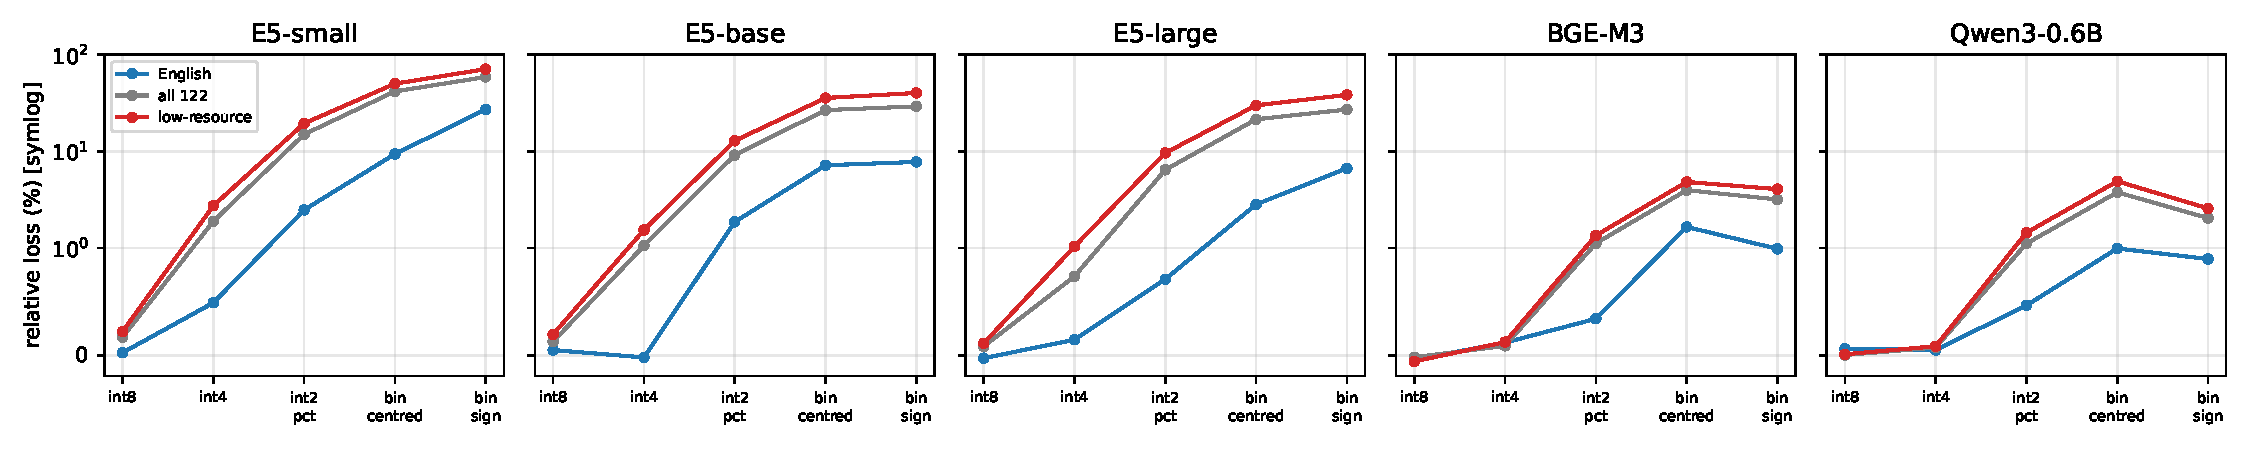
\includegraphics[width=\textwidth]{figs/fig2_loss_by_bits.pdf}
\caption{Relative loss by format for English, the mean over 122 languages and the mean over the 47 low-resource languages, per model. The vertical axis is symmetric-log, so both the near-zero losses at int8 and the large ones at 1 bit are visible.}\label{fig:bits}\end{figure}
Table~\ref{tab:drop} and Figure~\ref{fig:bits} give the loss per model for English, all languages, and low-resource languages. float16 changes nDCG@10 by at most 0.5\% in any language, and float8 and int8 by at most 0.5\% on average over languages; the largest single-language losses at int8 are 1--3\% and occur on languages the model already handles poorly. int4 costs E5-small 1.9\% on average and 2.7\% on low-resource languages, E5-base 1.1\%, and the other three models at most 0.7\%.

Below 4 bits the ordering English $<$ all languages $<$ low-resource holds in all five models and all formats. It is not driven by a few languages: with int2-clip, 98--99\% of the languages lose more than English for the E5 models and 80--85\% for BGE-M3 and Qwen3; with binary storage, 84--98\% and 87--91\%. The low-resource mean exceeds the all-language mean with non-overlapping bootstrap intervals for every model at binary (E5-small 70.9 [67.8, 73.9] vs.\ 58.8 [55.6, 62.0]; BGE-M3 4.1 [3.4, 4.8] vs.\ 3.2 [2.7, 3.7]). Excluding the languages on which a model fails outright at float32 (nDCG@10 $<0.3$; 2--8 per model) changes no entry of Table~\ref{tab:drop} by more than 1.5 points. Recall@10 gives the same picture (binary loss 48\%, 22\%, 20\%, 2\%, 2\% for the five models).

\subsection{How much is lost is decided by the model}\label{sec:model}
The magnitude differs by an order of magnitude between models. Under sign binarisation E5-small loses 27\% of nDCG@10 in English and 71\% on low-resource languages (Wolof, Guarani, Jingpho and romanised Sinhala 85--88\%); E5-base loses 8\% and 40\%; E5-large 7\% and 38\%; BGE-M3 1.0\% and 4.1\%; Qwen3 0.9\% and 2.6\%. The worst language for BGE-M3, romanised Urdu, loses 16\%, less than the best language for E5-small. E5-large has exactly the dimensionality of BGE-M3 and Qwen3, a higher float32 quality than Qwen3, and loses ten times more than either, so neither dimensionality nor float32 quality is what separates the models. Compressing the query as well raises every binary loss by 12--13 points for the E5 models and doubles it for BGE-M3 and Qwen3 (Appendix~\ref{app:sym}).

\subsection{The float32 margin explains the loss}\label{sec:margin}
\begin{figure}[t]\centering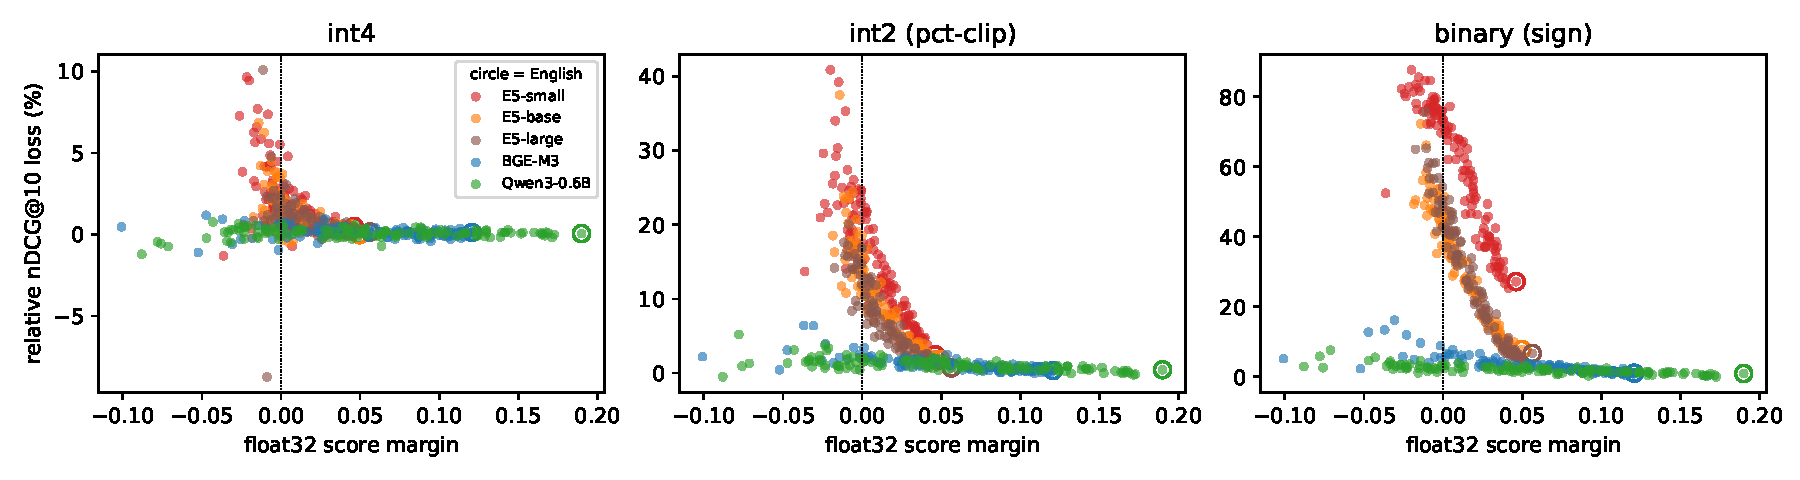
\includegraphics[width=\textwidth]{figs/fig1_loss_vs_margin.pdf}
\caption{Loss per language against the language's mean float32 margin, all five models, one point per language and model; circles mark English. Within each model the relation is monotone; between models the curves differ because the margins differ.}\label{fig:margin}\end{figure}
\begin{table}[t]\centering\footnotesize
\begin{tabular}{lrrrrrrr}
\toprule
model & $d$ & nDCG@10 & $\bar{c}$ & $\mu_{\mathrm{eng}}$ & $\mu_{\mathrm{low}}$ & $\rho_{\mathrm{bin}}$ & $\rho_{\mathrm{int2}}$ \\
\midrule
E5-small & 384 & 0.692 & 0.79 & 0.046 & -0.002 & -0.95 & -0.93 \\
E5-base & 768 & 0.736 & 0.78 & 0.050 & 0.003 & -0.98 & -0.96 \\
E5-large & 1024 & 0.785 & 0.77 & 0.056 & 0.008 & -0.98 & -0.96 \\
BGE-M3 & 1024 & 0.805 & 0.41 & 0.121 & 0.038 & -0.92 & -0.77 \\
Qwen3-0.6B & 1024 & 0.708 & 0.32 & 0.190 & 0.012 & -0.81 & -0.66 \\
\bottomrule
\end{tabular}
\caption{Embedding geometry per model. $\bar{c}$: mean cosine between passages (mean over languages); $\mu$: mean float32 margin for English and for low-resource languages; $\rho$: Spearman correlation across the 122 languages between margin and loss under binarisation / int2-clip.}\label{tab:geom}
\end{table}
Figure~\ref{fig:margin} plots the loss of every language against its mean float32 margin. Within each model the relation is monotone: the Spearman correlation between margin and binary loss is $-0.95$, $-0.98$, $-0.98$, $-0.92$ and $-0.81$ for E5-small, -base, -large, BGE-M3 and Qwen3, and $-0.93$, $-0.96$, $-0.96$, $-0.77$ and $-0.66$ for int2-clip (Table~\ref{tab:geom}). Between models the curves differ because the margins differ. The E5 embeddings are anisotropic at every size: the mean cosine between two unrelated documents is 0.77--0.79, so all scores live in a narrow band and the mean English margin is 0.05--0.06. In BGE-M3 and Qwen3 the mean document cosine is 0.41 and 0.32 and the English margin 0.12 and 0.19. Quantisation adds score noise of a size set by the format; rankings flip where the margin is smaller than the noise. Low-resource languages have the smallest margins in every model: in E5-small their mean margin is negative, i.e.\ the relevant document is on average not ranked first even at float32, and any noise costs.

\paragraph{Which languages are fragile is shared; how fragile is the model's.} The per-language margins of the five models agree closely (Spearman between models 0.90--0.98), and so do the per-language binary losses of the four encoder models (0.84--0.96; Qwen3, a decoder model, 0.57--0.70). The languages that a model embeds with thin margins are the same languages for every model; what the model decides is the scale.

\paragraph{Binarisation does not keep more of the vector in the robust models.} The cosine between an English float32 vector and its sign vector is 0.86 for E5-small and 0.77 for BGE-M3: the sign vector is a worse approximation for BGE-M3. What differs is the margin the noise has to overcome, so the relevant quantity is the margin relative to the noise of the format.

\paragraph{Covariates act through the margin.} Regressing the per-language loss on fertility, Latin script and Joshi class with model fixed effects over 575 model--language pairs gives $R^2=0.79$ for binary and $0.62$ for int2-clip. Joshi class is the strongest covariate ($-5.1$ points of binary loss per class, $p<0.001$), Latin script adds $+4.2$ points ($p=0.006$), and fertility is marginal ($p=0.07$), although fertility alone correlates with binary loss at $\rho=0.73$--$0.79$ for the encoder models (Figure~\ref{fig:fert}). The margin alone gives $R^2=0.74$ and $0.57$, and adding the three covariates to it raises $R^2$ by at most $0.06$. The covariates describe which languages a model embeds poorly; the margin measures it directly, without any metadata about the language.
\begin{figure}[t]\centering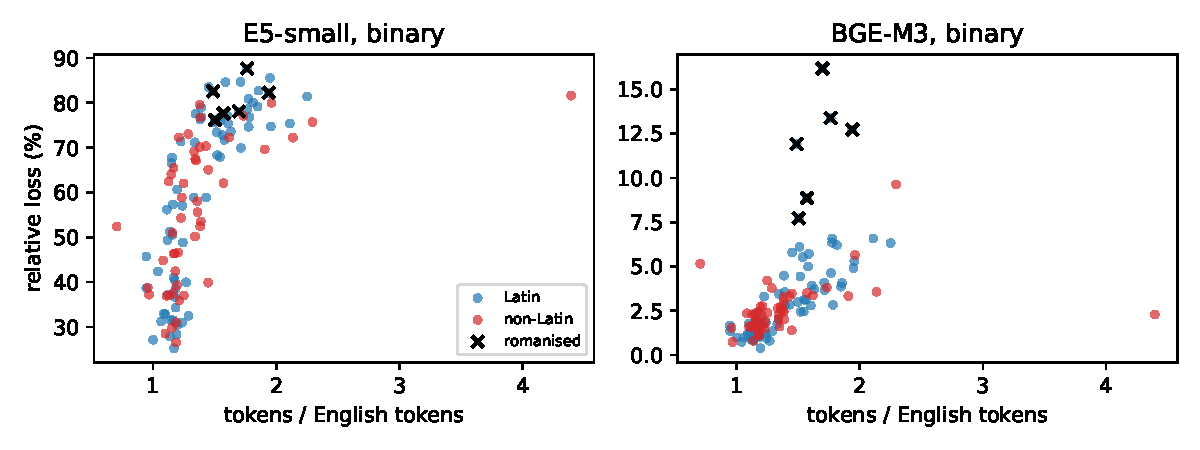
\includegraphics[width=0.75\textwidth]{figs/fig3_loss_vs_fertility.pdf}
\caption{Binary loss per language against tokenizer fertility (tokens relative to English for the same documents) for E5-small and BGE-M3; crosses are romanised variants. Fertility predicts the loss but with much more scatter than the margin, and the scale is again set by the model.}\label{fig:fert}\end{figure}

\paragraph{Same language, two scripts.} Six languages appear in their native script and romanised. Romanising the same Arabic, Bengali, Hindi, Nepali, Sinhala or Urdu text, with identical content, drives the E5 margin from $+0.01$--$0.03$ to between $-0.001$ and $-0.02$, the int2-clip loss from 4--10\% to 19--39\%, and the binary loss from 21--47\% to 60--80\% (Table~\ref{tab:script}). Script matters, but only through what it does to the margin.
\begin{table}[t]\centering\small
\begin{tabular}{llrrrrrr}\toprule
 & & \multicolumn{2}{c}{margin} & \multicolumn{2}{c}{int2-clip loss} & \multicolumn{2}{c}{binary loss} \\
language & script & native & Latin & native & Latin & native & Latin \\ \midrule
Arabic & Arab & 0.033 & -0.022 & 4.2 & 18.6 & 21.5 & 66.3 \\
Bengali & Beng & 0.022 & -0.007 & 6.6 & 27.2 & 35.4 & 65.7 \\
Hindi & Deva & 0.028 & -0.001 & 5.8 & 21.7 & 26.0 & 59.9 \\
Nepali & Deva & 0.014 & -0.012 & 10.4 & 23.1 & 45.2 & 68.8 \\
Sinhala & Sinh & 0.013 & -0.017 & 9.9 & 39.2 & 46.8 & 79.9 \\
Urdu & Arab & 0.015 & -0.014 & 10.3 & 28.7 & 43.4 & 68.3 \\ \bottomrule
\end{tabular}
\caption{Same language in its native script and romanised (E5-small and E5-base pooled): float32 margin and loss (\%).}\label{tab:script}
\end{table}

\subsection{The calibration language does not matter; the range estimator does}\label{sec:calib}
\begin{table}[t]\centering\footnotesize
\begin{tabular}{llrrrrr}
\toprule
scheme & languages & English & mixed (LOO) & Latin-only & target, 64 & target, all \\
\midrule
int2 & all 122 & 20.1 & 20.6 & 19.9 & 9.5 & 15.9 \\
 & low-res. & 27.3 & 27.7 & 26.8 & 12.6 & 20.6 \\
int2-clip & all 122 & 10.2 & 9.5 & 9.5 & 7.7 & 7.2 \\
 & low-res. & 14.0 & 13.0 & 13.1 & 10.4 & 9.8 \\
bin-centred & all 122 & 29.9 & 27.9 & 27.8 & 23.4 & 23.3 \\
 & low-res. & 38.6 & 35.6 & 35.4 & 30.1 & 30.1 \\
\bottomrule
\end{tabular}
\caption{Loss (\%) by calibration source, E5 models pooled; 1388 vectors except ``target, 64''; LOO = leave-target-language-out.}\label{tab:calib}
\end{table}
Table~\ref{tab:calib} isolates the calibration source on the three E5 models, the ones sensitive to it; Appendix~\ref{app:calib} has all five. Replacing English calibration by the mixed sample, which never contains the evaluated language, or by Latin-script languages only, changes the loss by at most 3.2 points in any row, and in both directions. Even the in-language oracle, which has seen the evaluation vectors, recovers only about a fifth of the int2 and of the centred-binary loss. The calibration language is not what makes the difference.

Two estimator choices matter more. First, clipping the range to the 5th--95th percentiles halves the mean and the low-resource int2 loss of every model (Table~\ref{tab:drop}: 29$\to$15\% for E5-small, 18$\to$9\% for E5-base, 13$\to$6\% for E5-large). The min/max range is stretched by outliers, so most of the four levels of int2 are wasted on values that never occur; this is also why 64 in-language calibration vectors give a lower min/max int2 loss than 1388 of them (10\% vs.\ 16\%), since a smaller sample has a narrower range. Second, centring each dimension before taking the sign cuts the binary loss of E5-small from 27\% to 9\% in English and from 71\% to 50\% on low-resource languages, because anisotropic embeddings share a large common component that a threshold at zero encodes identically into every vector, wasting the bit. Sixty-four target-language texts capture the in-language benefit of both fixes; 1388 add at most half a point.

\subsection{Subtracting the mean removes most of the loss}\label{sec:whiten}
\begin{table}[t]\centering\footnotesize
\begin{tabular}{llrrrrrrr}
\toprule
model & transform (calib.) & nDCG$_{32}$ & $\bar{c}$ & margin & bin all & bin low & bin vs.\ $\mathrm{nDCG}_{32}'$ & int2-clip all \\
\midrule
E5-small & none & 0.692 & 0.79 & 0.010 & 58.8 & 70.9 & 58.8 & 15.0 \\
 & centre (Eng) & 0.735 & 0.35 & 0.043 & 3.9 & 2.1 & 11.5 & -4.9 \\
 & centre (mixed) & 0.741 & 0.25 & 0.049 & 0.0 & -3.3 & 9.2 & -7.3 \\
 & ZCA (Eng) & 0.576 & 0.55 & -0.004 & 38.6 & 46.8 & 24.6 & 26.7 \\
 & ZCA (mixed) & 0.733 & 0.14 & 0.058 & -0.6 & -7.2 & 8.9 & -8.2 \\
\midrule
E5-base & none & 0.736 & 0.78 & 0.016 & 29.2 & 40.2 & 29.2 & 9.1 \\
 & centre (Eng) & 0.764 & 0.34 & 0.054 & 2.6 & 3.0 & 7.0 & -2.8 \\
 & centre (mixed) & 0.774 & 0.27 & 0.063 & -0.6 & -2.3 & 5.7 & -4.9 \\
 & ZCA (Eng) & 0.503 & 0.58 & -0.014 & 48.3 & 62.9 & 21.7 & 40.3 \\
 & ZCA (mixed) & 0.735 & 0.20 & 0.054 & 6.2 & 3.7 & 7.5 & 0.5 \\
\midrule
E5-large & none & 0.785 & 0.77 & 0.021 & 27.1 & 38.4 & 27.1 & 6.4 \\
 & centre (Eng) & 0.804 & 0.33 & 0.067 & 1.8 & 2.1 & 4.8 & -1.7 \\
 & centre (mixed) & 0.811 & 0.26 & 0.076 & -0.4 & -1.2 & 3.8 & -3.2 \\
 & ZCA (Eng) & 0.522 & 0.60 & -0.010 & 48.1 & 61.0 & 20.0 & 40.9 \\
 & ZCA (mixed) & 0.761 & 0.19 & 0.061 & 8.4 & 7.8 & 6.0 & 4.1 \\
\midrule
BGE-M3 & none & 0.805 & 0.41 & 0.064 & 3.2 & 4.1 & 3.2 & 1.1 \\
 & centre (Eng) & 0.808 & 0.18 & 0.092 & 1.9 & 2.6 & 2.4 & 0.3 \\
 & centre (mixed) & 0.809 & 0.15 & 0.094 & 1.6 & 2.1 & 2.2 & 0.0 \\
 & ZCA (Eng) & 0.732 & 0.17 & 0.058 & 15.4 & 18.3 & 6.2 & 11.5 \\
 & ZCA (mixed) & 0.769 & 0.07 & 0.077 & 8.7 & 9.7 & 4.1 & 5.8 \\
\midrule
Qwen3-0.6B & none & 0.708 & 0.32 & 0.055 & 2.0 & 2.6 & 2.0 & 1.1 \\
 & centre (Eng) & 0.713 & 0.13 & 0.071 & 0.6 & 0.7 & 1.5 & -0.3 \\
 & centre (mixed) & 0.713 & 0.11 & 0.071 & 0.5 & 0.3 & 1.5 & -0.4 \\
 & ZCA (Eng) & 0.671 & 0.20 & 0.044 & 8.7 & 9.4 & 3.7 & 6.0 \\
 & ZCA (mixed) & 0.715 & 0.09 & 0.072 & 1.3 & 0.8 & 2.8 & -0.9 \\
\bottomrule
\end{tabular}
\caption{Centring and whitening before compression. nDCG$_{32}$: float32 quality after the transform (mean over 122 languages); $\bar{c}$: mean passage cosine; margin: mean float32 margin. Losses are relative to the \emph{original} float32 quality, except the column marked vs.\ nDCG$_{32}'$, which is relative to the transformed float32 quality. Negative values are gains over the original float32 baseline.}\label{tab:whiten}
\end{table}
\begin{figure}[t]\centering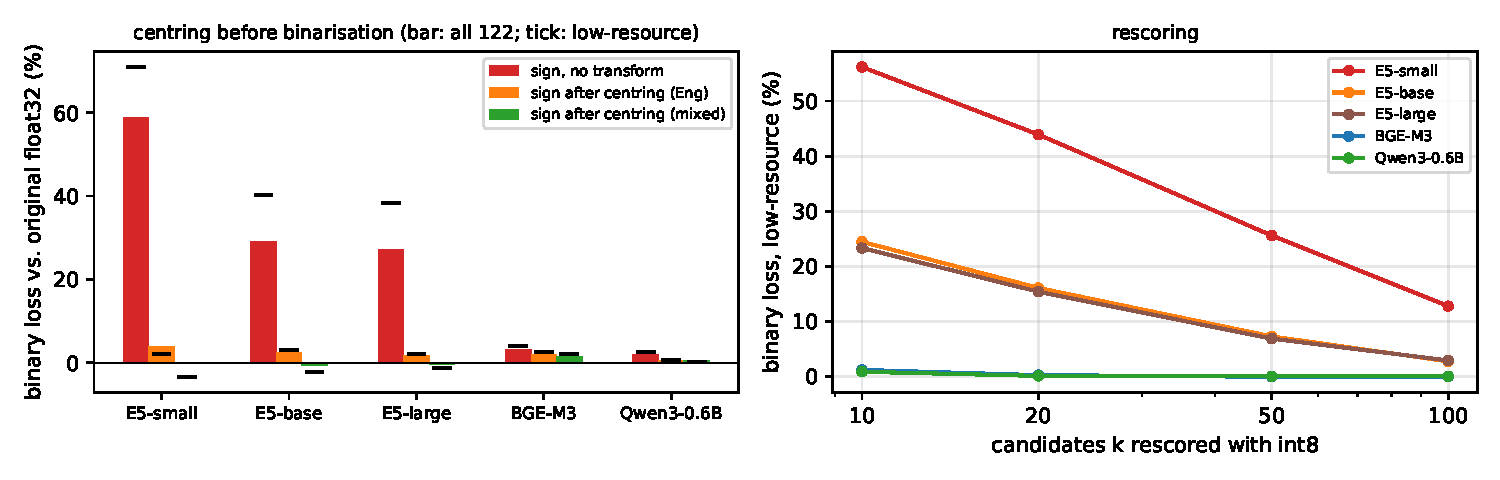
\includegraphics[width=\textwidth]{figs/fig4_centring_rescoring.pdf}
\caption{Left: binary loss relative to the original float32 quality before and after centring on the calibration mean, per model (bars: mean over 122 languages; ticks: low-resource mean). Right: binary loss on low-resource languages after rescoring $k$ candidates with an int8 corpus.}\label{fig:fix}\end{figure}
If the loss is caused by thin margins in a narrow cone, spreading the cone should remove it. Table~\ref{tab:whiten} and Figure~\ref{fig:fix} (left) test this directly. Subtracting the calibration mean, one $d$-dimensional vector fitted on English and applied unchanged to all 122 languages, transforms the E5 models. For E5-small the mean document cosine falls from 0.79 to 0.35, the mean margin rises from 0.010 to 0.043, the float32 quality itself improves from 0.692 to 0.735 nDCG@10, and the binary loss relative to the original float32 quality falls from 59\% to 3.9\% on average and from 71\% to 2.1\% on low-resource languages; int2-clip and int4 storage after centring are \emph{better} than the original float32 by 5 and 9 points. The same holds for E5-base and E5-large (binary loss 29$\to$2.6\% and 27$\to$1.8\%). Measured against the improved float32 baseline, the fair comparison, the residual binary loss is 11.5\%, 7.0\% and 4.8\%, down from 59\%, 29\% and 27\%. Centring changes BGE-M3 and Qwen3 by under a point, because their spaces are already spread. Centring on the mixed sample is marginally better than on English (E5-small: 0.0\% binary loss, $-7.2$\% on low-resource languages), so again the language of the calibration data is secondary.

Full ZCA whitening fitted on 1388 English vectors overfits: it lowers the float32 quality of every model (E5-small 0.692$\to$0.576) and raises every loss. Fitted on the more diverse mixed sample it matches centring for E5-small, falls short of it for the larger E5 models, and still hurts BGE-M3. The common component, not the full covariance, carries the damage, and removing it is enough.

This result closes the argument. The per-language inequality of Section~\ref{sec:uneven} is neither a property of the languages nor of the bit width: a translation of the embedding space by a single vector removes most of it, in every language, without any target-language data.

\subsection{Rescoring a short candidate list}\label{sec:rescore}
\begin{table}[t]\centering\footnotesize
\begin{tabular}{llrrrrrrrrrrrr}
\toprule
model & index & \multicolumn{3}{c}{$k=10$} & \multicolumn{3}{c}{$k=20$} & \multicolumn{3}{c}{$k=50$} & \multicolumn{3}{c}{$k=100$} \\
 & & Eng & all & low & Eng & all & low & Eng & all & low & Eng & all & low \\
\midrule
E5-small & binary & 13.1 & 43.6 & 56.2 & 7.9 & 32.8 & 43.9 & 3.3 & 18.4 & 25.6 & 1.4 & 9.0 & 12.8 \\
 & int2-clip & 0.2 & 6.3 & 8.5 & 0.0 & 2.8 & 3.8 & 0.1 & 0.6 & 0.8 & 0.0 & 0.3 & 0.3 \\
E5-base & binary & 2.3 & 16.6 & 24.4 & 1.3 & 10.5 & 16.1 & 0.2 & 4.6 & 7.3 & 0.2 & 1.7 & 2.7 \\
 & int2-clip & 0.1 & 3.3 & 5.0 & 0.0 & 1.3 & 1.9 & 0.0 & 0.3 & 0.4 & 0.0 & 0.1 & 0.2 \\
E5-large & binary & 2.7 & 15.4 & 23.3 & 1.2 & 9.9 & 15.4 & 0.4 & 4.3 & 6.9 & 0.1 & 1.7 & 2.9 \\
 & int2-clip & -0.1 & 2.2 & 3.4 & -0.1 & 0.7 & 1.1 & 0.0 & 0.2 & 0.4 & 0.0 & 0.2 & 0.3 \\
BGE-M3 & binary & 0.0 & 0.9 & 1.2 & 0.0 & 0.2 & 0.2 & 0.0 & 0.0 & -0.1 & 0.0 & 0.0 & -0.1 \\
 & int2-clip & -0.1 & 0.2 & 0.3 & 0.0 & 0.0 & 0.0 & 0.0 & 0.0 & -0.1 & 0.0 & 0.0 & -0.1 \\
Qwen3-0.6B & binary & 0.1 & 0.6 & 0.8 & 0.1 & 0.1 & 0.1 & 0.1 & 0.0 & 0.0 & 0.1 & 0.0 & 0.0 \\
 & int2-clip & 0.2 & 0.3 & 0.4 & 0.1 & 0.0 & 0.0 & 0.1 & 0.0 & 0.0 & 0.1 & 0.0 & 0.0 \\
\bottomrule
\end{tabular}
\caption{Loss (\%) after retrieving $k$ candidates with the compressed index and rescoring them with the float32 query against an int8 corpus. Rescoring with the float32 corpus differs by at most 0.2 points. English calibration.}\label{tab:rescore}
\end{table}
Table~\ref{tab:rescore} and Figure~\ref{fig:fix} (right) give the loss after retrieving $k$ candidates with the compressed index and rescoring them with the float32 query against an int8 copy of the corpus; rescoring against the float32 corpus differs by at most 0.2 points, so the int8 copy is sufficient. Note that $k=10$ already reorders the ten retrieved documents, which is why its loss is below that of Table~\ref{tab:drop}. Rescoring works, but the number of candidates it needs is again set by the model and the language. For BGE-M3 and Qwen3, 20 candidates remove the binary loss everywhere. For the E5 models the loss decays roughly geometrically in $k$, and 100 candidates still leave 9\% on average and 13\% on low-resource languages for E5-small (E5-base and -large: 2--3\%). With the int2-clip index, 50 candidates suffice for every model and language group (at most 0.8\%). In storage terms, a binary index plus an int8 copy costs 9/32 of float32, while centred binary alone costs 1/32 and, for the E5 models, loses less. Centring is the cheaper and the stronger fix, and the two combine.

\subsection{A second task with larger corpora}\label{sec:wiki}
\begin{table}[t]\centering\footnotesize
\begin{tabular}{llrrrrrrr}
\toprule
model & task & nDCG & margin & int2-clip & bin-sign & bin-centred & $\rho_{\mathrm{bin}}$ \\
\midrule
E5-small & Wikipedia & 0.877 & 0.025 & 3.4 & 27.1 & 18.8 & -0.54 \\
 & Belebele & 0.906 & 0.034 & 5.5 & 33.9 & 23.1 & -0.86 \\
E5-base & Wikipedia & 0.888 & 0.027 & 1.4 & 5.6 & 6.5 & -0.78 \\
 & Belebele & 0.927 & 0.039 & 3.0 & 10.8 & 11.2 & -0.69 \\
E5-large & Wikipedia & 0.908 & 0.031 & 0.8 & 3.1 & 3.9 & -0.60 \\
 & Belebele & 0.948 & 0.044 & 1.8 & 7.7 & 7.5 & -0.83 \\
BGE-M3 & Wikipedia & 0.899 & 0.079 & 0.2 & 1.2 & 0.8 & -0.50 \\
 & Belebele & 0.935 & 0.110 & 0.6 & 1.4 & 1.9 & -0.51 \\
Qwen3-0.6B & Wikipedia & 0.868 & 0.082 & 0.4 & 1.0 & 1.4 & -0.67 \\
 & Belebele & 0.899 & 0.134 & 0.6 & 1.1 & 2.0 & -0.60 \\
\bottomrule
\end{tabular}
\caption{Wikipedia (13.5k passages per language) vs.\ Belebele, same 16 languages: mean loss (\%); $\rho$ = Spearman(margin, binary loss).}\label{tab:wiki}
\end{table}
To check that the model ordering is not a property of Belebele's small corpus, we repeat the protocol on the Wikipedia retrieval task of MTEB: 16 languages, 13{,}500 passages and 1{,}500 queries each, 28 times more passages per language (Table~\ref{tab:wiki}; the Belebele rows are restricted to the same 16 languages). The ordering is unchanged (binary: E5-small 27\%, E5-base 6\%, E5-large 3\%, BGE-M3 and Qwen3 about 1\%) and the loss on the larger corpus is equal to or smaller than on Belebele for every model and format. The margin ordering within models persists ($\rho$ from $-0.50$ to $-0.83$ for binary), weaker than on Belebele because these mostly high-resource European languages span a narrow range of margins. Per-language losses of the E5 models agree across the two tasks (Spearman 0.67--0.77 over the 16 languages); for BGE-M3 and Qwen3 the losses are within a point of zero on both tasks and their ranking is noise.

\section{Recommendations}\label{sec:reco}
For a practitioner storing multilingual embeddings on a device, the results reduce to five rules.
\begin{enumerate}[nosep]
\item \textbf{int8 and int4 are safe} for every model and language tested; use them without further checks.
\item \textbf{Below 4 bits, measure the margin first.} Embed a few hundred labelled queries per language of interest at float32 and compute the mean margin. Languages with a margin below about 0.02 for E5-type models will lose heavily under 1--2 bit storage; languages with a margin above 0.1 will not.
\item \textbf{Subtract the calibration mean before compressing}, and re-normalise. The vector can be fitted on English. For anisotropic models this alone removes most of the loss and improves float32 retrieval as well.
\item \textbf{Clip integer ranges to percentiles} rather than using the sample minimum and maximum, and keep the query in float.
\item \textbf{Do not expect multilingual calibration to help.} The language of the calibration text changes the loss by a few points at most; the estimator and the centring change it by tens of points.
\end{enumerate}

\section{Discussion and limitations}
\paragraph{Why the inequality is a model property.} A low-resource language loses more because the model embeds it worse: its relevant documents sit closer to the distractors, so any noise flips more rankings. This is the same mechanism that makes English lose more in E5-small than in BGE-M3, and the same mechanism that centring acts on. Compression does not create the inequality; it exposes an inequality in margins that is invisible at float32 as long as the relevant document is still ranked first. Reporting float32 quality alone hides it, and reporting compressed quality on English alone hides it entirely.

\paragraph{Limitations.} Both tasks have one relevant document per query and short passages; tasks with graded relevance or long documents may behave differently, although the margin argument applies to any noise added to scores. The larger corpus covers 16 mostly high-resource languages. We evaluate scalar formats only; product quantisation and learned codebooks have their own calibration and were not tested. Models were run at their released checkpoints without fine-tuning for compression, and a model trained with compression in mind may not show the effect. The Joshi classes date from 2020 and are missing for seven dialects. Finally, the margin threshold in Recommendation~2 is read off Figure~\ref{fig:margin} for these models and formats and should be recalibrated for others.

\section{Broader impact statement}
The paper documents a way in which a routine engineering choice, storing embeddings at low precision, degrades search quality for speakers of low-resource languages far more than for speakers of English, and shows that the degradation is invisible in the English-only evaluations that are standard practice. It also shows that a fix costing one vector removes most of the damage. We see no direct negative use. The measurement protocol requires labelled queries in each language, which exist for the 122 Belebele languages but not for most of the world's languages; for those, the margin cannot be computed and the loss cannot be verified.

\section{Conclusion}
At 2 and 1 bit per dimension, compressed multilingual embeddings lose retrieval quality unevenly: English least, low-resource languages most, in every model tested. Whether the loss is 3\% or 70\% is decided by the model's embedding geometry, not by the bit width, the dimensionality or the language of the calibration data. The float32 score margin predicts the loss per language, explains why anisotropic models collapse while isotropic ones do not, and points to the remedy that works: subtract the mean, clip the ranges, keep the query in float.

\subsubsection*{Reproducibility statement}
All embeddings are computed once and stored; every format, calibration source, transform and rescoring variant is applied in NumPy to the stored vectors, and every table and figure in this paper is produced by a script from the released per-language result files. Code, result files and scripts are at \url{https://anonymous.4open.science/r/embedding-compression-languages-23FB}. Total compute: about 6 GPU-hours on a single T4 for embedding, and under one CPU-hour on a laptop for everything else.

\bibliography{main}
\bibliographystyle{tmlr}

\appendix
\section{Compressing the query as well}\label{app:sym}
\begin{table}[t]\centering\footnotesize
\begin{tabular}{lrrrrrr}
\toprule
model & \multicolumn{2}{c}{int4} & \multicolumn{2}{c}{int2-clip} & \multicolumn{2}{c}{binary} \\
 & query fp32 & query compressed & query fp32 & query compressed & query fp32 & query compressed \\
\midrule
E5-small & 1.9 & 2.2 & 15.0 & 19.0 & 58.8 & 70.5 \\
E5-base & 1.1 & 1.2 & 9.1 & 12.1 & 29.2 & 41.8 \\
E5-large & 0.7 & 0.9 & 6.4 & 8.7 & 27.1 & 39.4 \\
BGE-M3 & 0.1 & 0.1 & 1.1 & 2.0 & 3.2 & 6.5 \\
Qwen3-0.6B & 0.1 & 0.1 & 1.1 & 1.8 & 2.0 & 4.4 \\
\bottomrule
\end{tabular}
\caption{Mean relative loss (\%) over 122 languages when only the corpus is compressed (query float32) versus when the query is compressed the same way.}\label{tab:sym}
\end{table}

Table~\ref{tab:sym} compares compressing only the corpus, the setting of the main text, with compressing the query in the same format.

\section{Calibration source, all models}\label{app:calib}
\begin{table}[t]\centering\footnotesize
\begin{tabular}{lllrrrrr}
\toprule
model & scheme & languages & English & mixed (LOO) & Latin-only & target, 64 & target, all \\
\midrule
E5-small & int2 & all & 29.3 & 29.9 & 28.2 & 14.4 & 23.7 \\
 &  & low-res. & 37.9 & 38.2 & 35.9 & 18.0 & 29.1 \\
 & int2-clip & all & 15.0 & 13.4 & 13.9 & 11.8 & 11.2 \\
 &  & low-res. & 19.4 & 17.5 & 18.3 & 15.2 & 14.8 \\
 & bin-centred & all & 41.7 & 39.9 & 40.0 & 34.8 & 34.6 \\
 &  & low-res. & 50.1 & 47.6 & 47.6 & 42.7 & 42.7 \\
\midrule
E5-base & int2 & all & 17.8 & 18.3 & 18.4 & 8.4 & 14.0 \\
 &  & low-res. & 24.6 & 25.5 & 25.6 & 11.6 & 18.8 \\
 & int2-clip & all & 9.1 & 8.8 & 8.6 & 6.6 & 6.2 \\
 &  & low-res. & 12.8 & 12.4 & 12.0 & 8.9 & 8.4 \\
 & bin-centred & all & 26.7 & 24.2 & 24.0 & 20.2 & 20.2 \\
 &  & low-res. & 35.7 & 31.9 & 31.4 & 26.2 & 26.1 \\
\midrule
E5-large & int2 & all & 13.3 & 13.5 & 13.1 & 5.8 & 9.9 \\
 &  & low-res. & 19.4 & 19.4 & 18.8 & 8.2 & 13.8 \\
 & int2-clip & all & 6.4 & 6.2 & 6.0 & 4.7 & 4.2 \\
 &  & low-res. & 9.6 & 9.1 & 8.9 & 7.1 & 6.2 \\
 & bin-centred & all & 21.5 & 19.5 & 19.4 & 15.2 & 15.2 \\
 &  & low-res. & 29.9 & 27.3 & 27.2 & 21.5 & 21.4 \\
\midrule
BGE-M3 & int2 & all & 2.7 & 2.8 & 2.7 & 1.5 & 2.6 \\
 &  & low-res. & 3.5 & 3.7 & 3.4 & 2.0 & 3.4 \\
 & int2-clip & all & 1.1 & 1.2 & 1.2 & 1.4 & 1.3 \\
 &  & low-res. & 1.3 & 1.4 & 1.4 & 1.9 & 1.6 \\
 & bin-centred & all & 4.0 & 3.9 & 4.0 & 4.1 & 4.1 \\
 &  & low-res. & 4.8 & 4.8 & 4.8 & 5.3 & 5.3 \\
\midrule
Qwen3-0.6B & int2 & all & 2.3 & 2.4 & 2.3 & 1.2 & 2.2 \\
 &  & low-res. & 2.8 & 3.2 & 3.0 & 1.5 & 2.8 \\
 & int2-clip & all & 1.1 & 1.1 & 1.2 & 1.4 & 1.3 \\
 &  & low-res. & 1.4 & 1.5 & 1.6 & 1.9 & 1.8 \\
 & bin-centred & all & 3.8 & 3.9 & 3.9 & 4.3 & 4.3 \\
 &  & low-res. & 4.9 & 5.1 & 5.3 & 5.8 & 5.7 \\
\bottomrule
\end{tabular}
\caption{Loss (\%) by calibration source for every model (1388 vectors except ``target, 64''; LOO = leave-target-language-out).}\label{tab:calib_full}
\end{table}

\section{Per-language results}\label{app:perlang}
Table~\ref{tab:perlang} lists, for every language, the loss under binary and int2-clip storage for each model. Per-language results for all formats, calibration sources, transforms and query modes, together with margins, fertility and geometry statistics, are in the released CSV files.
\begin{small}
\begin{longtable}{llrrrrrrrrrrr}
\caption{Per-language float32 margin ($\mu$) and relative loss (\%) under binarisation (bin) and int2-clip (int2) for every model; J = Joshi class.}\label{tab:perlang}\\
\toprule
language & script & J & \multicolumn{2}{c}{E5-small} & \multicolumn{2}{c}{E5-base} & \multicolumn{2}{c}{E5-large} & \multicolumn{2}{c}{BGE-M3} & \multicolumn{2}{c}{Qwen3-0.6B} \\
 & & & bin & int2 & bin & int2 & bin & int2 & bin & int2 & bin & int2 \\
\midrule
\endfirsthead
\toprule
language & script & J & \multicolumn{2}{c}{E5-small} & \multicolumn{2}{c}{E5-base} & \multicolumn{2}{c}{E5-large} & \multicolumn{2}{c}{BGE-M3} & \multicolumn{2}{c}{Qwen3-0.6B} \\
 & & & bin & int2 & bin & int2 & bin & int2 & bin & int2 & bin & int2 \\
\midrule
\endhead
\bottomrule
\endfoot
Mesopotamian Arabic & Arab & -- & 47 & 8 & 19 & 4 & 14 & 3 & 2 & 0 & 1 & 1 \\
Afrikaans & Latn & 3 & 61 & 12 & 22 & 4 & 24 & 3 & 2 & 1 & 2 & 1 \\
Tosk Albanian & Latn & 1 & 59 & 14 & 27 & 7 & 17 & 3 & 2 & 0 & 2 & 1 \\
Amharic & Ethi & 2 & 69 & 22 & 36 & 11 & 36 & 7 & 3 & 1 & 4 & 2 \\
North Levantine Arabic & Arab & -- & 51 & 10 & 16 & 4 & 18 & 3 & 2 & 1 & 0 & 0 \\
Standard Arabic & Arab & 5 & 31 & 5 & 12 & 3 & 6 & 2 & 1 & 0 & 1 & 0 \\
Arabic (romanised) & Latn & 5 & 82 & 21 & 50 & 16 & 65 & 14 & 13 & 3 & 3 & 1 \\
Najdi Arabic & Arab & -- & 39 & 9 & 17 & 4 & 10 & 2 & 3 & 1 & 1 & 1 \\
Moroccan Arabic & Arab & -- & 62 & 22 & 30 & 7 & 39 & 7 & 4 & 2 & 2 & 1 \\
Egyptian Arabic & Arab & 3 & 46 & 11 & 25 & 6 & 20 & 4 & 2 & 0 & 1 & 0 \\
Assamese & Beng & 1 & 70 & 21 & 39 & 9 & 35 & 8 & 3 & 2 & 3 & 1 \\
North Azerbaijani & Latn & 1 & 68 & 11 & 27 & 7 & 25 & 5 & 2 & 0 & 1 & 1 \\
Bambara & Latn & 1 & 80 & 19 & 45 & 13 & 47 & 15 & 6 & 2 & 1 & 1 \\
Bengali & Beng & 3 & 54 & 8 & 17 & 5 & 19 & 4 & 2 & 1 & 2 & 1 \\
Bengali (romanised) & Latn & 3 & 78 & 35 & 54 & 19 & 50 & 15 & 9 & 2 & 3 & 2 \\
Tibetan & Tibt & 1 & 52 & 14 & 66 & 15 & 52 & 16 & 5 & 2 & 6 & 5 \\
Bulgarian & Cyrl & 3 & 30 & 6 & 10 & 3 & 7 & 2 & 2 & 0 & 1 & 1 \\
Catalan & Latn & 4 & 40 & 7 & 13 & 2 & 7 & 2 & 1 & 0 & 1 & 0 \\
Cebuano & Latn & 3 & 68 & 19 & 33 & 10 & 34 & 7 & 2 & 0 & 1 & 1 \\
Czech & Latn & 4 & 31 & 4 & 8 & 2 & 6 & 2 & 2 & 0 & 1 & 1 \\
Central Kurdish & Arab & 1 & 76 & 25 & 53 & 20 & 49 & 15 & 10 & 2 & 3 & 2 \\
Danish & Latn & 3 & 33 & 5 & 10 & 3 & 6 & 2 & 2 & 1 & 1 & 1 \\
German & Latn & 5 & 25 & 4 & 10 & 2 & 6 & 1 & 1 & 0 & 0 & 0 \\
Greek & Grek & 3 & 40 & 8 & 14 & 4 & 6 & 2 & 1 & 0 & 1 & 0 \\
English & Latn & 5 & 27 & 2 & 8 & 2 & 7 & 1 & 1 & 0 & 1 & 0 \\
Estonian & Latn & 3 & 37 & 8 & 14 & 4 & 10 & 2 & 2 & 0 & 3 & 0 \\
Basque & Latn & 4 & 51 & 12 & 18 & 4 & 11 & 3 & 2 & 0 & 3 & 2 \\
Finnish & Latn & 4 & 31 & 5 & 9 & 3 & 5 & 1 & 1 & 1 & 2 & 1 \\
French & Latn & 5 & 32 & 6 & 11 & 2 & 6 & 1 & 1 & 0 & 1 & 0 \\
Nigerian Fulfulde & Latn & 0 & 84 & 27 & 51 & 22 & 61 & 17 & 6 & 2 & 3 & 2 \\
West Central Oromo & Latn & 1 & 81 & 30 & 51 & 24 & 54 & 17 & 6 & 2 & 5 & 1 \\
Guarani & Latn & 1 & 85 & 23 & 51 & 14 & 49 & 17 & 4 & 1 & 1 & 1 \\
Gujarati & Gujr & 1 & 70 & 15 & 39 & 10 & 32 & 6 & 3 & 2 & 2 & 1 \\
Haitian Creole & Latn & 2 & 79 & 21 & 45 & 14 & 47 & 8 & 3 & 2 & 3 & 2 \\
Hausa & Latn & 2 & 77 & 19 & 34 & 12 & 35 & 12 & 4 & 1 & 3 & 2 \\
Hebrew & Hebr & 3 & 37 & 7 & 15 & 5 & 8 & 2 & 1 & 0 & 2 & 1 \\
Hindi & Deva & 4 & 37 & 7 & 15 & 5 & 11 & 2 & 2 & 1 & 1 & 0 \\
Hindi (romanised) & Latn & 4 & 76 & 25 & 44 & 19 & 47 & 13 & 8 & 2 & 1 & 2 \\
Croatian & Latn & 4 & 56 & 9 & 12 & 4 & 9 & 2 & 1 & 1 & 2 & 0 \\
Hungarian & Latn & 4 & 39 & 8 & 11 & 2 & 6 & 1 & 1 & 1 & 1 & 0 \\
Armenian & Armn & 1 & 70 & 22 & 37 & 16 & 40 & 9 & 3 & 1 & 2 & 2 \\
Igbo & Latn & 1 & 75 & 27 & 51 & 17 & 43 & 12 & 7 & 2 & 3 & 1 \\
Ilocano & Latn & 1 & 77 & 19 & 37 & 11 & 35 & 10 & 3 & 1 & 1 & 1 \\
Indonesian & Latn & 3 & 39 & 6 & 7 & 2 & 7 & 2 & 1 & 0 & 1 & 1 \\
Icelandic & Latn & 2 & 57 & 15 & 24 & 8 & 13 & 4 & 2 & 1 & 2 & 1 \\
Italian & Latn & 4 & 30 & 4 & 9 & 3 & 8 & 2 & 0 & 0 & 0 & 0 \\
Javanese & Latn & 1 & 67 & 13 & 33 & 8 & 31 & 6 & 2 & 1 & 3 & 2 \\
Japanese & Jpan & 5 & 37 & 6 & 10 & 2 & 7 & 2 & 2 & 1 & 1 & 1 \\
Jingpho & Latn & 0 & 86 & 30 & 56 & 12 & 57 & 14 & 5 & 1 & 2 & 1 \\
Kannada & Knda & 1 & 56 & 12 & 25 & 7 & 18 & 4 & 3 & 0 & 1 & 1 \\
Georgian & Geor & 3 & 67 & 22 & 35 & 12 & 25 & 5 & 2 & 1 & 3 & 1 \\
Kazakh & Cyrl & 3 & 64 & 16 & 32 & 9 & 31 & 7 & 2 & 1 & 2 & 1 \\
Kabuverdianu & Latn & -- & 78 & 26 & 53 & 16 & 42 & 7 & 3 & 3 & 2 & 1 \\
Halh Mongolian & Cyrl & 1 & 72 & 17 & 38 & 15 & 41 & 9 & 3 & 1 & 3 & 2 \\
Khmer & Khmr & 1 & 72 & 23 & 47 & 14 & 46 & 13 & 3 & 1 & 3 & 2 \\
Kinyarwanda & Latn & 1 & 70 & 21 & 34 & 8 & 34 & 5 & 4 & 1 & 2 & 2 \\
Kyrgyz & Cyrl & 1 & 66 & 17 & 29 & 11 & 28 & 6 & 2 & 1 & 3 & 1 \\
Korean & Hang & 4 & 38 & 6 & 11 & 3 & 7 & 2 & 2 & 0 & 1 & 1 \\
Lao & Laoo & 2 & 77 & 24 & 35 & 21 & 35 & 12 & 3 & 1 & 3 & 3 \\
Lingala & Latn & 1 & 73 & 15 & 51 & 13 & 37 & 12 & 4 & 1 & 4 & 1 \\
Lithuanian & Latn & 3 & 41 & 9 & 13 & 3 & 7 & 2 & 1 & 1 & 2 & 1 \\
Ganda & Latn & 1 & 77 & 17 & 48 & 13 & 57 & 9 & 6 & 3 & 2 & 1 \\
Luo & Latn & -- & 76 & 21 & 47 & 17 & 42 & 10 & 6 & 1 & 2 & 1 \\
Standard Latvian & Latn & 3 & 49 & 13 & 16 & 4 & 8 & 2 & 1 & 0 & 2 & 1 \\
Malayalam & Mlym & 1 & 52 & 9 & 24 & 5 & 16 & 2 & 2 & 1 & 2 & 1 \\
Marathi & Deva & 2 & 54 & 11 & 22 & 8 & 16 & 2 & 2 & 0 & 2 & 1 \\
Macedonian & Cyrl & 1 & 46 & 11 & 12 & 4 & 8 & 2 & 1 & 0 & 2 & 1 \\
Maltese & Latn & 2 & 75 & 16 & 35 & 8 & 38 & 5 & 5 & 2 & 2 & 2 \\
Maori & Latn & 1 & 83 & 22 & 48 & 18 & 60 & 13 & 4 & 2 & 3 & 0 \\
Burmese & Mymr & 1 & 77 & 25 & 37 & 13 & 33 & 8 & 4 & 1 & 1 & 1 \\
Dutch & Latn & 4 & 28 & 5 & 11 & 2 & 6 & 1 & 1 & 0 & 1 & 0 \\
Norwegian Bokmal & Latn & 1 & 31 & 4 & 11 & 3 & 6 & 2 & 1 & 0 & 1 & 1 \\
Nepali & Deva & 1 & 62 & 13 & 28 & 8 & 21 & 5 & 2 & 1 & 3 & 1 \\
Nepali (romanised) & Latn & 1 & 83 & 23 & 55 & 24 & 61 & 16 & 12 & 4 & 3 & 2 \\
Northern Sotho & Latn & 1 & 79 & 18 & 47 & 14 & 42 & 13 & 5 & 2 & 1 & 0 \\
Nyanja & Latn & 1 & 72 & 23 & 42 & 11 & 42 & 10 & 5 & 1 & 3 & 2 \\
Odia & Orya & 1 & 65 & 14 & 27 & 8 & 21 & 3 & 3 & 1 & 2 & 2 \\
Eastern Panjabi & Guru & -- & 62 & 18 & 32 & 11 & 26 & 4 & 4 & 1 & 2 & 1 \\
Southern Pashto & Arab & 1 & 80 & 21 & 44 & 11 & 42 & 7 & 3 & 1 & 4 & 3 \\
Western Persian & Arab & 4 & 29 & 5 & 10 & 3 & 7 & 2 & 2 & 1 & 1 & 1 \\
Plateau Malagasy & Latn & 1 & 73 & 19 & 39 & 9 & 32 & 8 & 3 & 1 & 4 & 2 \\
Polish & Latn & 4 & 34 & 6 & 10 & 4 & 7 & 2 & 1 & 1 & 1 & 1 \\
Portuguese & Latn & 4 & 49 & 9 & 15 & 4 & 10 & 3 & 1 & 1 & 1 & 0 \\
Romanian & Latn & 3 & 31 & 5 & 8 & 2 & 6 & 1 & 1 & 1 & 1 & 0 \\
Russian & Cyrl & 4 & 27 & 5 & 8 & 2 & 6 & 1 & 1 & 1 & 0 & 0 \\
Shan & Mymr & 0 & 82 & 39 & 49 & 19 & 57 & 20 & 2 & 0 & 3 & -1 \\
Sinhala (romanised) & Latn & 0 & 88 & 41 & 72 & 37 & 76 & 18 & 13 & 6 & 6 & 3 \\
Sinhala & Sinh & 0 & 67 & 12 & 27 & 8 & 22 & 5 & 2 & 0 & 3 & 4 \\
Slovak & Latn & 3 & 40 & 7 & 9 & 2 & 6 & 2 & 1 & 0 & 1 & 1 \\
Slovenian & Latn & 3 & 51 & 8 & 14 & 3 & 8 & 3 & 1 & 0 & 2 & 1 \\
Shona & Latn & 1 & 74 & 25 & 40 & 13 & 42 & 8 & 4 & 1 & 2 & 1 \\
Sindhi & Arab & 1 & 73 & 23 & 39 & 17 & 35 & 8 & 4 & 1 & 2 & 2 \\
Somali & Latn & 1 & 76 & 29 & 44 & 16 & 49 & 15 & 4 & 2 & 3 & 1 \\
Southern Sotho & Latn & 1 & 75 & 18 & 47 & 14 & 41 & 11 & 7 & 2 & 3 & 2 \\
Spanish & Latn & 5 & 28 & 5 & 8 & 2 & 5 & 1 & 2 & 1 & 0 & 0 \\
Serbian & Cyrl & 4 & 42 & 9 & 11 & 3 & 8 & 2 & 1 & 1 & 2 & 1 \\
Swati & Latn & 1 & 75 & 19 & 45 & 12 & 51 & 13 & 4 & 1 & 3 & 2 \\
Sundanese & Latn & 1 & 71 & 17 & 41 & 12 & 27 & 5 & 3 & 1 & 2 & 0 \\
Swedish & Latn & 4 & 33 & 5 & 10 & 3 & 5 & 2 & 1 & 1 & 1 & 1 \\
Swahili & Latn & 2 & 57 & 12 & 19 & 4 & 17 & 4 & 2 & 1 & 2 & 2 \\
Tamil & Taml & 3 & 58 & 11 & 23 & 6 & 17 & 3 & 3 & 0 & 2 & 1 \\
Telugu & Telu & 1 & 50 & 11 & 21 & 6 & 23 & 4 & 2 & 1 & 2 & 1 \\
Tajik & Cyrl & 1 & 72 & 14 & 41 & 18 & 41 & 12 & 4 & 1 & 2 & 1 \\
Tagalog & Latn & 3 & 59 & 12 & 24 & 7 & 19 & 4 & 3 & 1 & 1 & 0 \\
Thai & Thai & 3 & 45 & 10 & 16 & 4 & 9 & 2 & 2 & 1 & 1 & 0 \\
Tigrinya & Ethi & 2 & 80 & 23 & 49 & 24 & 47 & 14 & 6 & 3 & 8 & 1 \\
Tswana & Latn & 2 & 79 & 17 & 48 & 12 & 51 & 9 & 4 & 2 & 1 & 2 \\
Tsonga & Latn & 1 & 77 & 17 & 45 & 12 & 45 & 10 & 3 & 1 & 2 & 1 \\
Turkish & Latn & 4 & 42 & 6 & 8 & 3 & 8 & 2 & 1 & 0 & 2 & 0 \\
Ukrainian & Cyrl & 3 & 36 & 5 & 9 & 3 & 6 & 1 & 2 & 1 & 1 & 0 \\
Urdu & Arab & 3 & 59 & 13 & 28 & 7 & 19 & 5 & 2 & 1 & 2 & 1 \\
Urdu (romanised) & Latn & 3 & 78 & 34 & 58 & 23 & 65 & 16 & 16 & 6 & 2 & 2 \\
Northern Uzbek & Latn & 3 & 71 & 18 & 33 & 12 & 26 & 6 & 2 & 1 & 2 & 2 \\
Vietnamese & Latn & 4 & 37 & 8 & 8 & 2 & 6 & 2 & 1 & 0 & 0 & 0 \\
Waray & Latn & 1 & 68 & 15 & 28 & 9 & 29 & 6 & 2 & 0 & 1 & 1 \\
Wolof & Latn & 2 & 85 & 25 & 56 & 17 & 61 & 14 & 6 & 3 & 2 & 1 \\
Xhosa & Latn & 2 & 76 & 24 & 40 & 11 & 41 & 9 & 3 & 2 & 3 & 2 \\
Yoruba & Latn & 2 & 81 & 26 & 46 & 11 & 53 & 8 & 6 & 2 & 3 & 2 \\
Chinese (Simplified) & Hans & 5 & 37 & 8 & 12 & 4 & 18 & 5 & 1 & 0 & 0 & 0 \\
Chinese (Traditional) & Hant & 5 & 39 & 7 & 11 & 3 & 24 & 6 & 2 & 0 & 0 & 0 \\
Standard Malay & Latn & 3 & 46 & 6 & 11 & 3 & 11 & 1 & 2 & 0 & 0 & 1 \\
Zulu & Latn & 2 & 76 & 25 & 47 & 10 & 45 & 8 & 3 & 1 & 4 & 2 \\
\end{longtable}
\end{small}

\end{document}
